\documentclass[10pt, conference]{IEEEtran}

\IEEEoverridecommandlockouts
% The preceding line is only needed to identify funding in the first footnote. If that is unneeded, please comment it out.
\usepackage{cite}
\usepackage{amsmath,amssymb,amsfonts}
\usepackage{algorithmic}
\usepackage{graphicx}
\usepackage{textcomp}
\usepackage{xcolor}
\usepackage{capt-of}
\usepackage{cuted} 
\usepackage{float} 
\usepackage{dblfloatfix}
\usepackage{blindtext}
\usepackage{booktabs}
\usepackage{svg}
\usepackage{tikz}
\usepackage{bondgraphs}

\usepackage{lipsum,parskip,booktabs,graphicx,tabulary,tabularx}

\usepackage{subcaption}


\newcommand\MyLogo{%
  
\includegraphics[width=3cm]{logo.png}% Adjust the width as needed
}

\title{Study and development of an ergonomic\\
haptic interface using flexible coils}
\author{
  \textbf{Candidate:} Morgan CASALE\\

  \begin{minipage}[t]{0.4\textwidth}
    \begin{flushleft}
      
      \textbf{Supervisors:}\\
      Alessandro RIZZO (PoliTO)\\
      Domenico PRATTICHIZZO (UniSi)
    \end{flushleft}    
  \end{minipage}
  \hfill
  \begin{minipage}[t]{0.4\textwidth}
    \begin{flushright}
      \textbf{Co-supervisors:}\\
      Tommaso LISINI BALDI (UniSi)\\
      Leonardo FRANCO (UniSi)
    \end{flushright}
  \end{minipage}
}


\usepackage{tikz}    
\begin{document}
\maketitle
\begin{tikzpicture}[remember picture,overlay]
  \node[anchor=north east,inner sep=5pt] at (current page.north east)
  {
\includegraphics[scale=0.05]{logo.png}};
\end{tikzpicture}


\begin{abstract}
    This thesis aims to explore the use of flexible PCB coils in haptic applications to create realistic touch sensations. Current piezo actuators, commonly used for generating vibratory cues, have limitations such as limited low-frequency responses and lack of flexibility, which are crucial for realistic and wearable haptic interfaces. Flexible PCB coils, capable of producing low-frequency vibrations and withstanding bending stresses, offer a potential solution. The thesis will first create a mathematical model of the force transmission chain of a voice actuator-style haptic device created with flexible coils, considering also how the human finger reacts to its stimuli. It will then present the necessary electronics for driving the device and conclude with the design and testing of prototypes to evaluate the technology's potential and limitations.
\end{abstract}

\section{Physic's Model Study}
The haptic device we tried to develop for this thesis is at its heart a \textbf{multi-physical system}, where electrical, magnetic, and mechanical components interact with each other.
Voice coil actuators are characterized by three main components: a \textbf{coil}, a \textbf{magnet}, and a \textbf{membrane}. The coil generates a magnetic field when a \textbf{current flows} through it and by interacting with the magnetic field generated by the magnet, \textbf{creates a force} that moves the membrane. The membrane is then used to \textbf{transmit this force} to the user's finger, which can feel the force as a \textbf{vibration}.
In this section, we will try to create a complete model to explain its behavior using \textbf{bond graphs}.
\begin{figure}[H]
    \centering
    \resizebox{1\linewidth}{!}{
        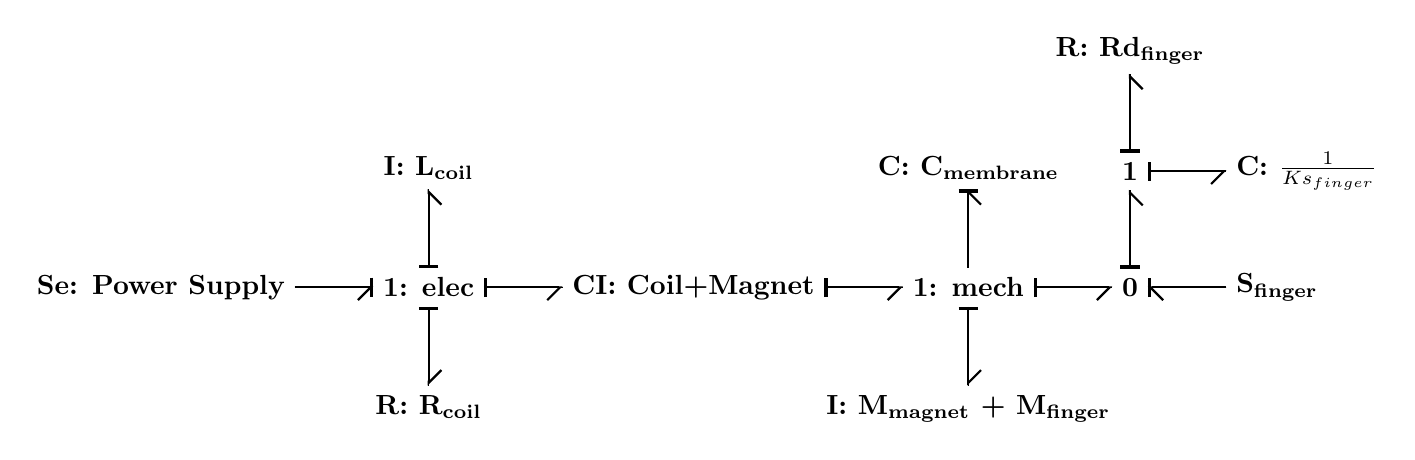
\begin{tikzpicture}
    \begin{scope}[every node/.style={bgelement}]
    \node (Se) at (0,0) {Se: Power Supply};
    \node[right=1 of Se] (i) {1: elec};
    \node[above=1 of i] (Iel) {I: L\textsubscript{coil}};
    \node[below=1 of i] (Rel) {R: R\textsubscript{coil}};
    \node[right=1 of i] (CI) {CI: Coil+Magnet};
    \node[right=1 of CI] (w1) {1: mech};
    \node[above=1 of w1] (Cm) {C: C\textsubscript{membrane}};
    \node[below=1 of w1] (Im) {I: M\textsubscript{magnet} + M\textsubscript{finger}};
    \node[right=1 of w1] (v) {0};
    \node[above=1 of v] (w2) {1};
    \node[above=1 of w2] (Rdf) {R: Rd\textsubscript{finger}};
    \node[right=1 of w2] (Cf) {C: $\frac{1}{Ks_{finger}}$};
    \node[right=1 of v] (Sfa) {S\textsubscript{finger}};
    \end{scope}
    \draw[bonds]
    (Se) edge [e_out] (i)
    (i) edge [e_in] (Iel)
    edge [e_in] (Rel)
    edge [e_in] (CI)
    (CI) edge [e_in] (w1)
    (w1) edge [e_out] (Cm)
    edge [e_in] (Im)
    (w1) edge [e_in] (v)
    (v) edge [e_in] (w2)
    (w2) edge [e_in] (Rdf)
    (w2) edge [e_in] (Cf)
    (Sfa) edge [e_out] (v);
\end{tikzpicture}
    
    } % TODO: Da fare bene
    \caption{Bond graph of the entire system, including the finger.}
    \label{fig: Total_bond-graph}
\end{figure}

\subsection{Electrical and Power Aspects of Coils}
The electrical part consists of the \textbf{voltage power supply} and the coil which is modeled as a \textbf{resistor} and an \textbf{inductor} in series. For this research, we're using planar concentric coils built using \textbf{flexible PCB technology}, this allows us freedom of design in creating a \textbf{flexible actuator}.
Due to their nature, these coils are very thin, which results in \textbf{high resistance} and \textbf{high heat production}. The power flowing through the coil must be \textbf{kept low to avoid damaging it}. This in turn means that the magnetic field generated by the coil will be \textbf{weak}, which can be a problem when trying to create strong haptic feedback.

\subsection{Electro-mechanical Transducer}
The electrical energy is converted into mechanical motion through the \textbf{magnetic repulsion force} between the coil and magnet, so the system acts as a \textbf{transducer}.
\begin{figure}[H]
    \centering
    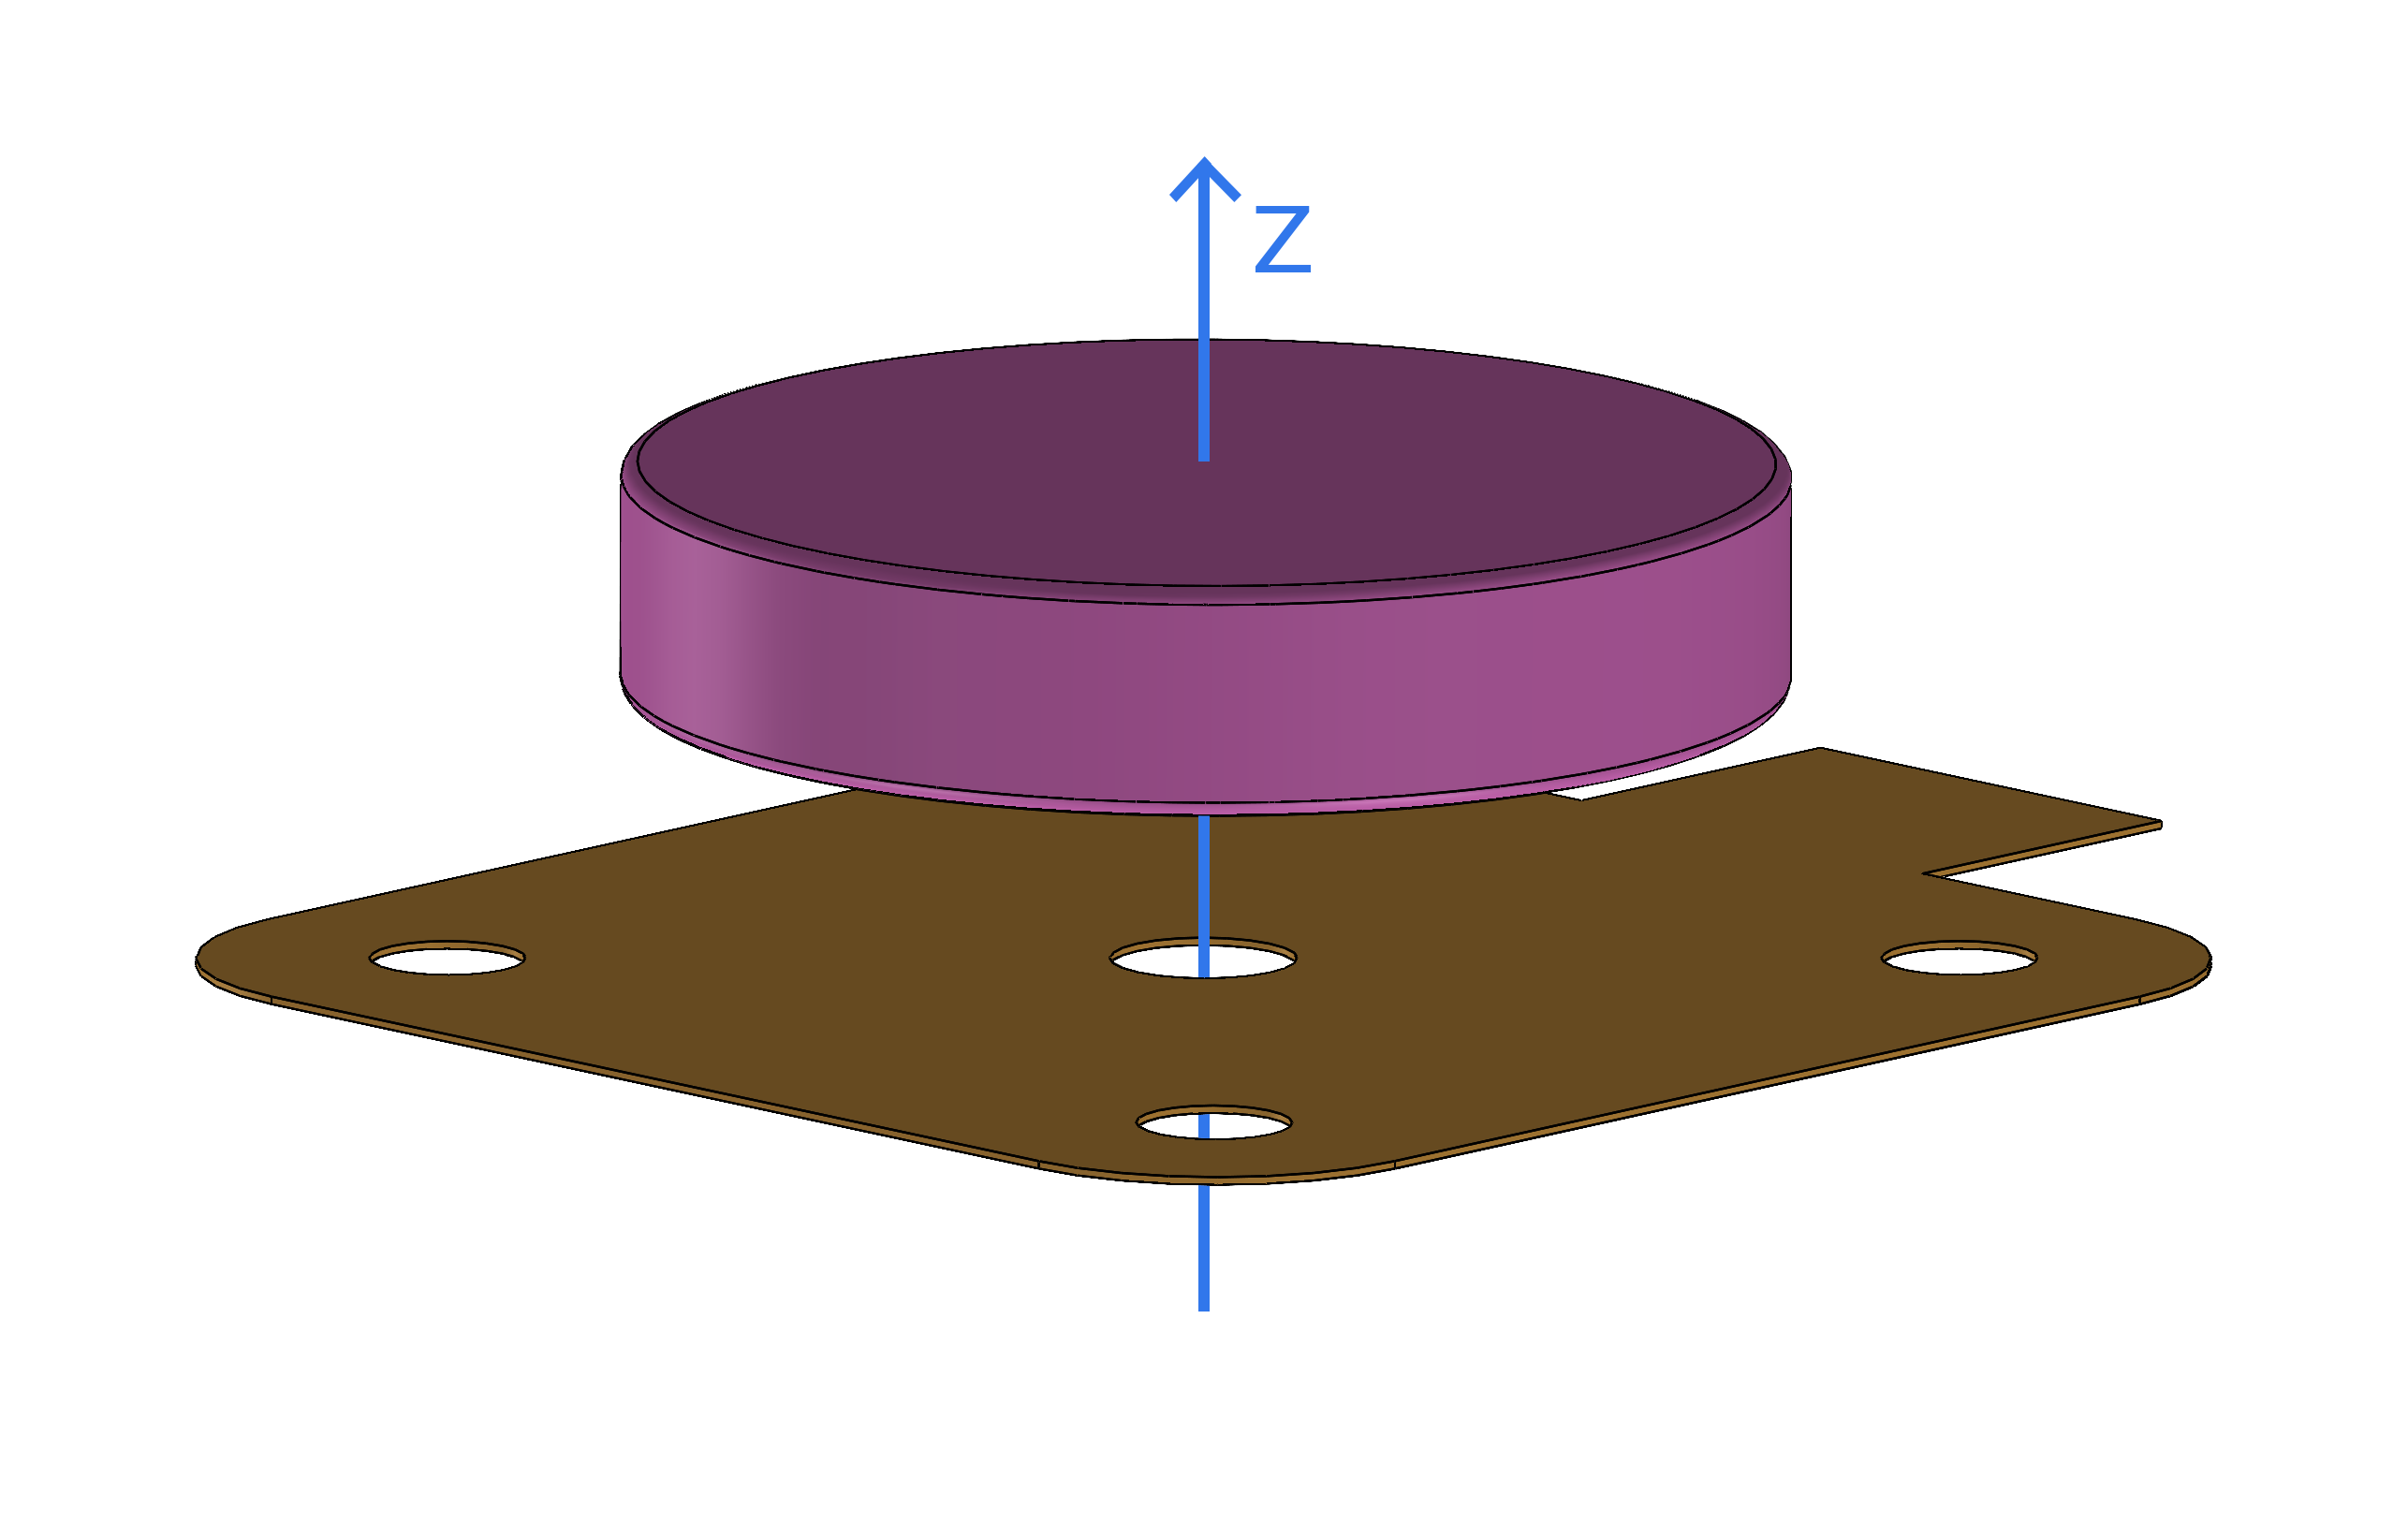
\includegraphics[width=0.4\columnwidth]{Figures/coil_magnet.png} 
    \caption[Coil-Magnet position]{Coil and magnet position in space.}
\end{figure}
The force is calculated through the \textbf{magnetic levitation} equation between the magnetic moment of the magnet and the magnetic field generated by planar windings:
\begin{equation*}
    F = \nabla (\overrightarrow{m_M} \cdot \overrightarrow{B_C}) = \frac{d}{dz} \left( \frac{B_M(z)}{\mu} \cdot \frac{\mu N I R_C^2}{2(R_C^2+z^2)^\frac{3}{2}} \right)
\end{equation*}

\subsection{Mechanical Membrane}
To limit the motion of the magnet only to the z-axis the magnet is inserted in a \textbf{flexible membrane}, this membrane is also used to \textbf{transmit the force} generated by the magnet to the user's finger.
For the last prototype, we designed a \textbf{celtic-cross-shaped silicone membrane} where the magnet is inserted in the center of the cross.
\begin{figure}[H]
    \centering
    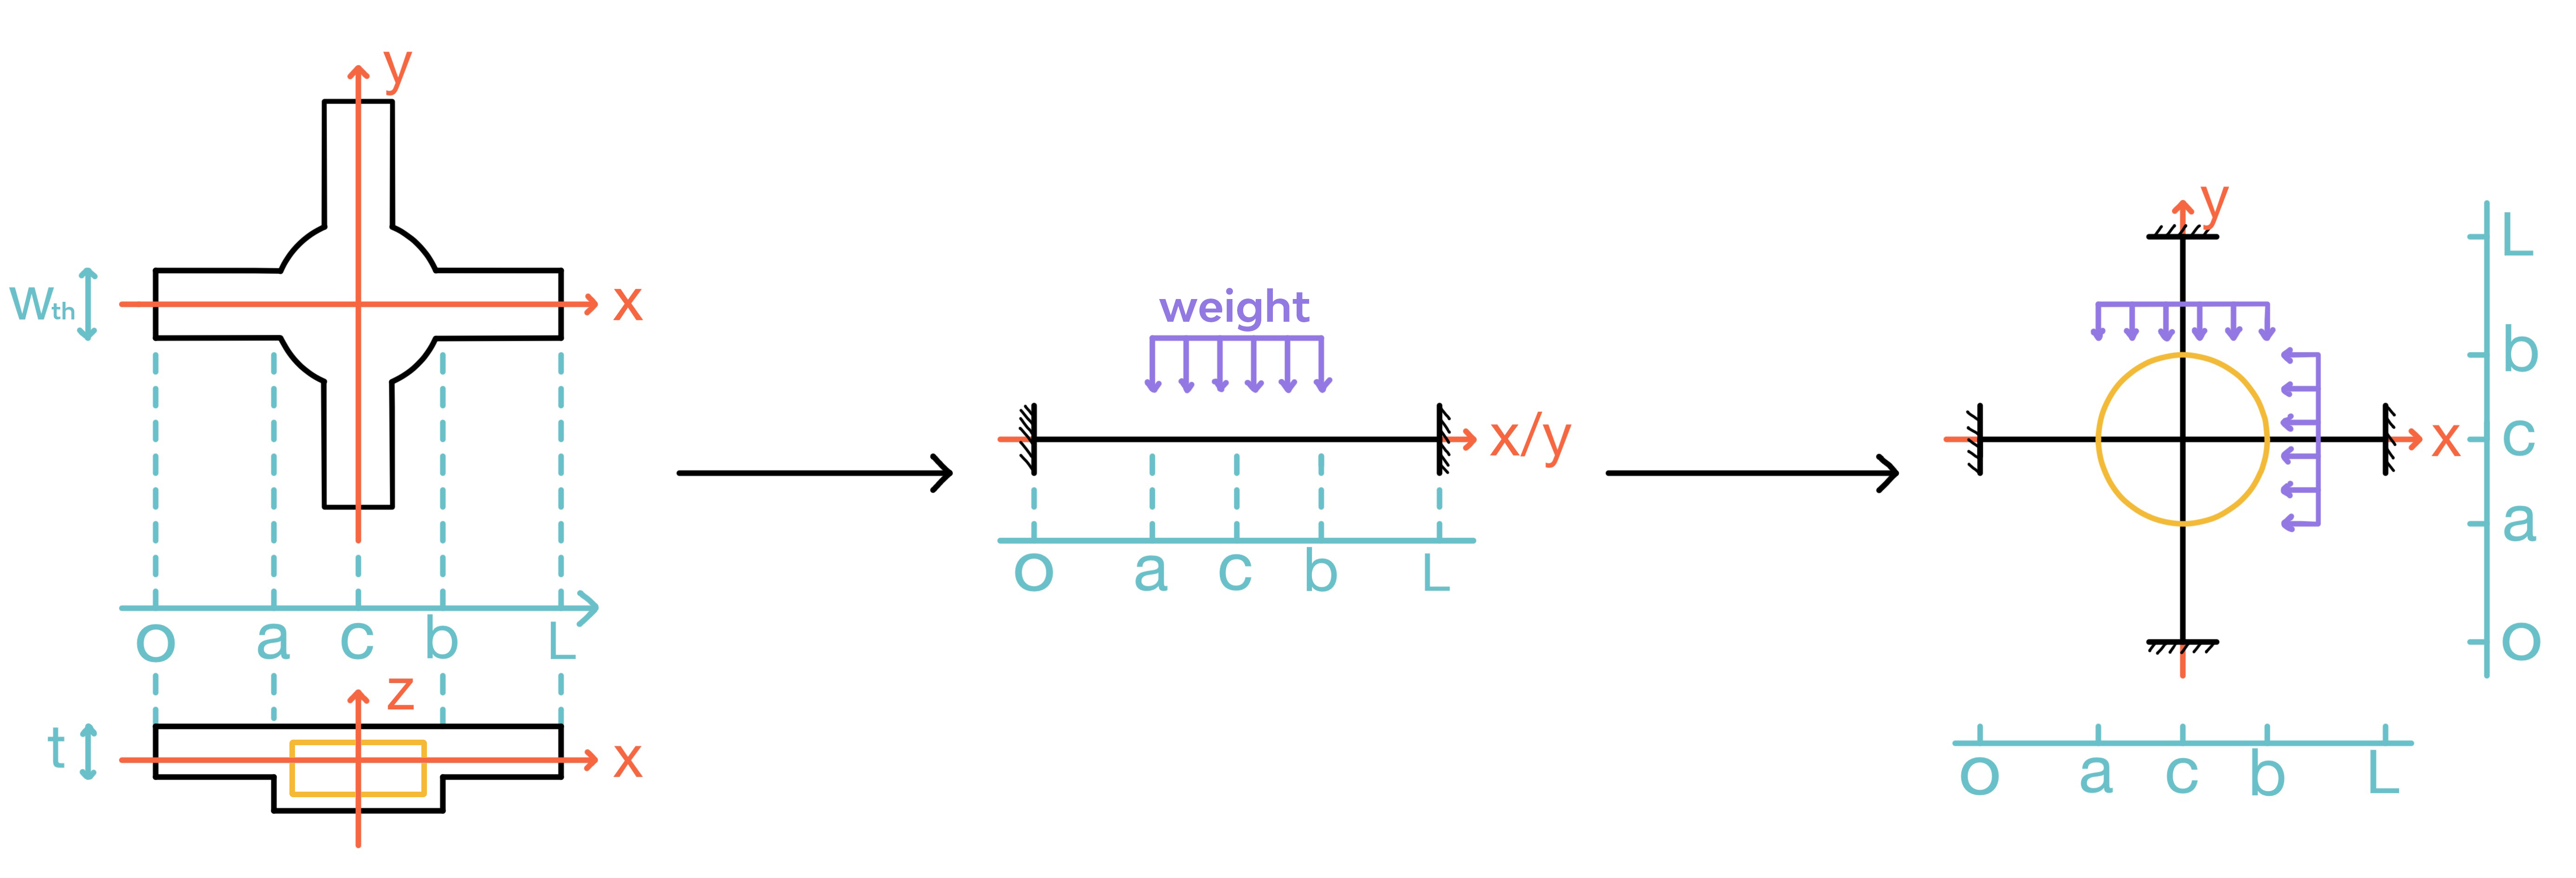
\includegraphics[width=0.9\linewidth]{Figures/membr_mech_model.jpg} 
    \caption[Membrane structure]{Membrane's structure and mechanical model.}
\end{figure}
The membrane can be modeled as a \textbf{spring-damper system}, where the spring represents the stiffness of the membrane, and the damping is negligible.
Finally, the finger grasping the membrane can also be modeled as a \textbf{mass-spring-damper} system where the inertia component is represented by the finger's mass, while the spring and damper represent respectively the stiffness and damping effects of the finger's skin.


\section{Haptics Overview}
Haptic Feedback is the research field that deals with the need to be able to \textbf{digitalize the human sense} of touch and \textbf{reproduce it}.
As this sense is \textbf{very complex} we still don’t understand it fully and we are \textbf{still not able to emulate it completely}. 
The human tactile sensing system can \textbf{measure specific properties of materials}, such as temperature, texture, force, friction, hardness and viscoelasticity, \textbf{through physical contact} between the human skin and the object.
Even the \textbf{changing state of the interaction}, such as gravitational and inertial effects, can be perceived through the sense of touch.
The sense of touch is based on the somatosensory system, which is composed of four main types of receptors, each one is specialized in detecting a specific type of stimulus: \textbf{mechanoreceptors, thermoreceptors, nociceptors and proprioceptors}.
Mechanoreceptors are the most important receptors for haptic feedback, as they are responsible for detecting \textbf{vibration and pressure}.
Their \textbf{sensitivity is limited} in both the frequency and amplitude of vibrations they can detect. The force amplitude limit also depends on the \textbf{constant pressure} applied to the skin.

\section{Device Control Unit}
Using coils to produce magnetic fields of usable intensity requires running them at pretty high currents.
This is because the magnetic field strength is proportional to the current flowing through the coil.
The goal of our device is to generate vibrations at different frequencies so we need to develop an AC-capable power supply.
Standard AC circuits are usually built to generate only low-current signals (in the order of tens of $mA$) but we need to generate signals in the order of $1A$.
For this reason, the control unit we are going to use has in its signal path a power amplifier based on power op-amps. Power op-amps have an integrated power stage that allows them to deliver high currents with a wide frequency bandwidth.
The signal can be generated through a microcontroller with a built-in DAC, in our case we tested the system with an ESP32 board.

\section{Implementation and Prototypes}
\subsection{Rigid Prototype}
The first prototype was designed to test the capabilities of coils produced by the \textbf{HZDR research group}.
In the previous research done by the HZDR team, they tested the coil using a simple piece of \textbf{flexible magnetic tape} as a membrane and magnet.
This membrane is shaped like a "fish" so the tail can be fixed on a plane and the head can be free to bend up and down.
\begin{figure}[H]
    \centering
    
\includegraphics[width = 0.2\linewidth]{Figures/Dresden_test.png}
    \caption{Dresden coil HZDR test setup}
    \label{fig: Dresden_test}
\end{figure}
The pulp needed to be \textbf{suspended} at a certain distance to avoid pressing and stopping the membrane.

To solve this problem we developed a structure able to fulfill this requirement.
\begin{figure}[H]
    \centering
    \begin{subcaptiongroup}
      \centering
      \parbox[b]{0.2\textwidth}{
        \centering
        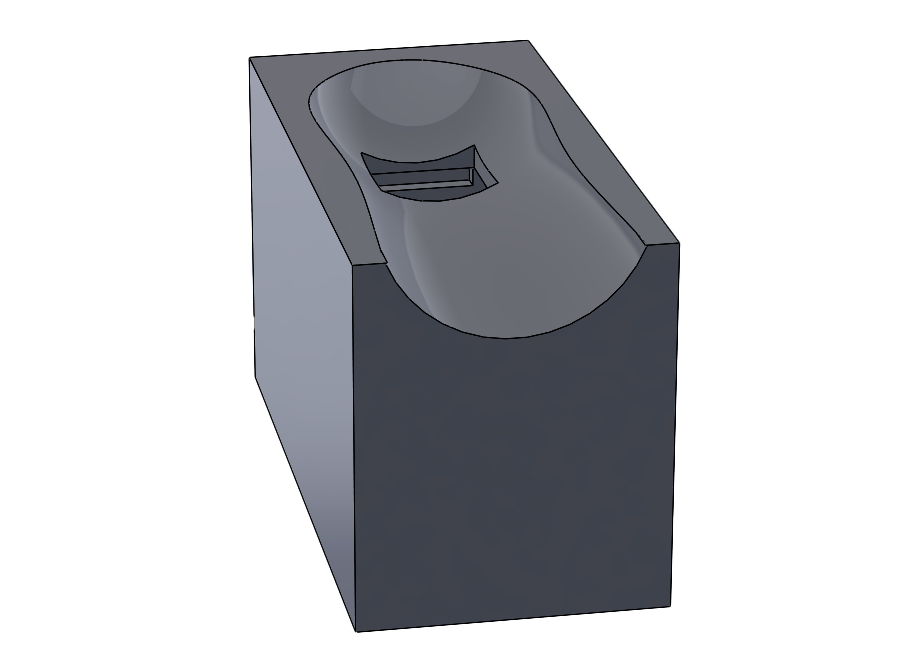
\includegraphics[width = 0.9\linewidth]{Figures/finger_holder.png}
        \caption{Finger resting surface}
      }
      \parbox[b]{0.2\textwidth}{
        \centering
        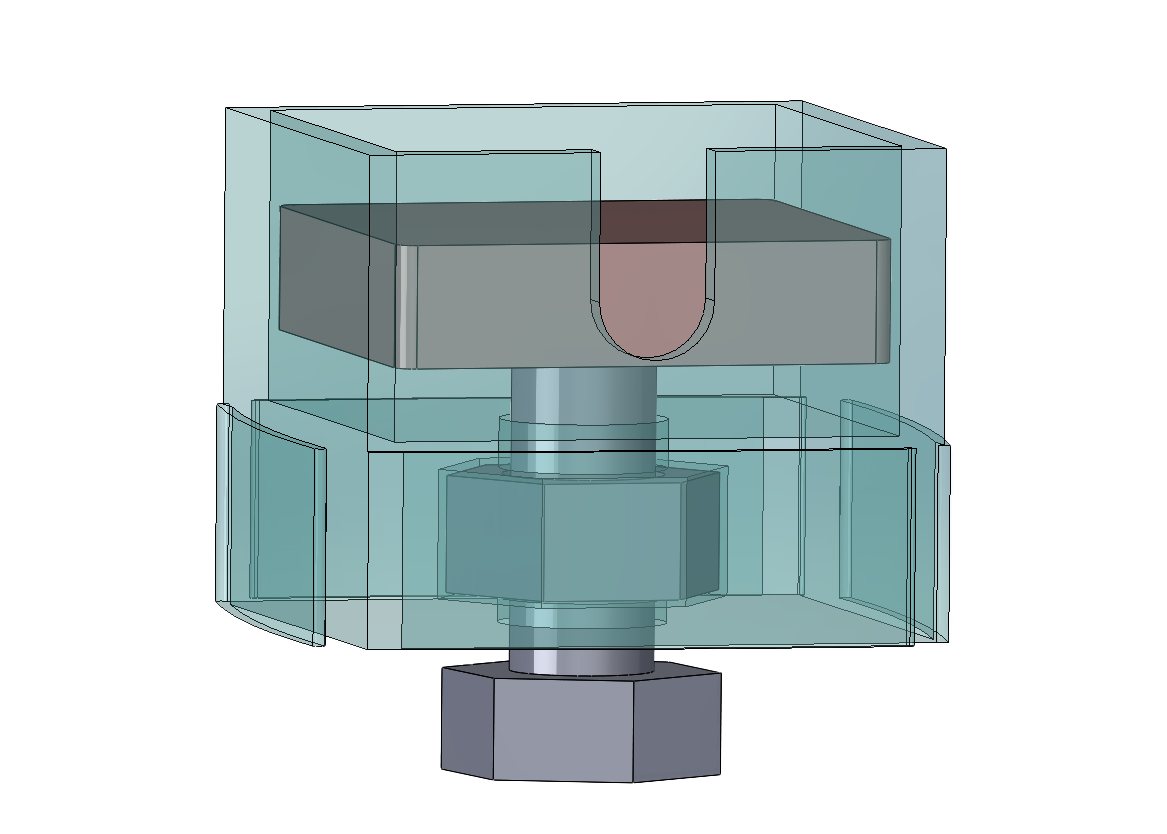
\includegraphics[width = 0.9\linewidth]{Figures/adj_platform.png}
        \caption{Finger platform}
      }
    \end{subcaptiongroup}
    \caption{Components of the first prototype}
\end{figure}
The coil and membrane are placed on top of the \textbf{height-adjustable platform}, to feel the vibrations the finger would lay on the hole of the resting surface.
We quickly moved on from this prototype as the coil was not able to generate \textbf{enough force} to be felt by the user because its \textbf{low power rating} limited its capability to generate a \textbf{strong enough magnetic field}.

\subsection{Wearable Rigid Prototype}
The following prototype was based on the flexible PCB coils. 
These have a \textbf{higher power rating}, can be \textbf{easily designed and manufactured} and are \textbf{sturdier} than the previous ones, especially under flexing conditions. 
A structure was designed to keep the coil in place and allow it to be \textbf{worn on the finger} through the use of silicon sleeves.
This sleeve was designed to be \textbf{adaptable to different finger sizes} and to \textbf{integrate a cylindrical magnet} on the pulp.
\begin{figure}[H]
    \centering
    \begin{subcaptiongroup}
        \centering
        \parbox[b]{0.2\textwidth}{
            \centering
            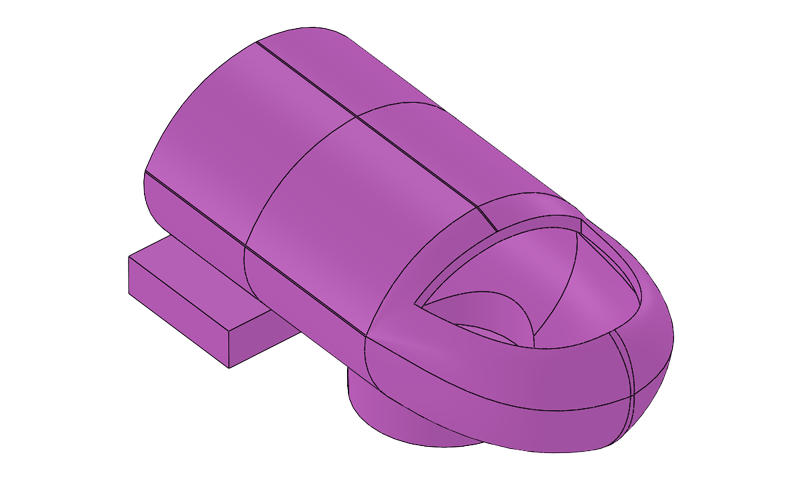
\includegraphics[width=0.2\textwidth]{Figures/silicon_sleeve_front.png}
        }
        \parbox[b]{0.2\textwidth}{
            \centering
            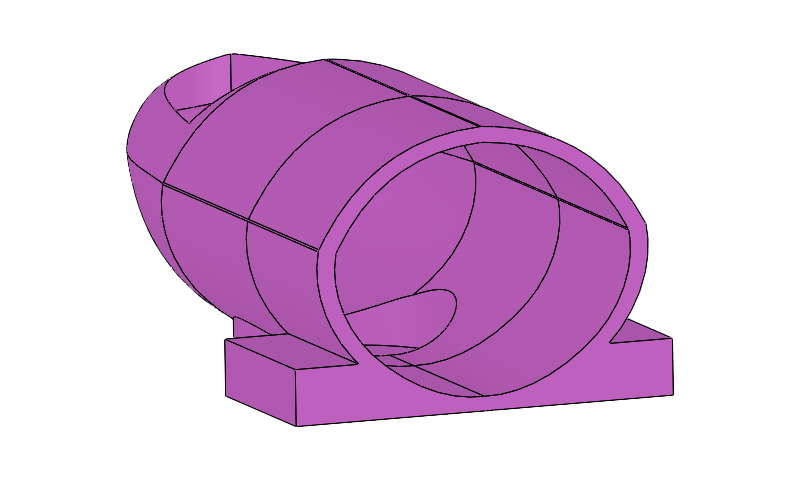
\includegraphics[width=0.2\textwidth]{Figures/silicon_sleeve_back.png}        
        }
    \end{subcaptiongroup}
    \caption{Finger silicon sleeve front and back view}
\end{figure}
The silicon sleeve could be then connected to the assembly where the coil and a heatsink were placed through its lateral mounting wings.
\begin{figure}[H]
    \centering
    \begin{subcaptiongroup}
        \centering
        \parbox[b]{0.2\textwidth}{
            \centering
            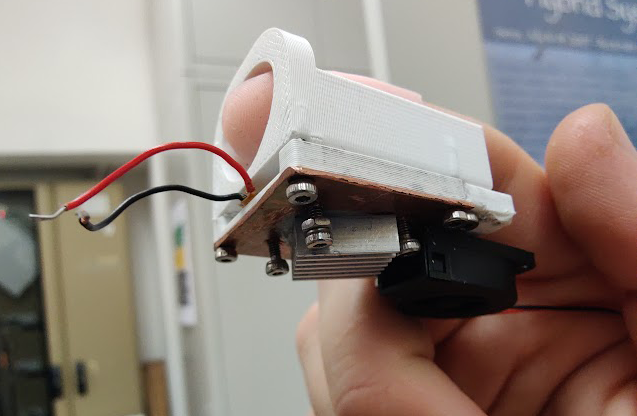
\includegraphics[width=0.2\textwidth]{Figures/rigid_prot_btm.png}
        }
        \parbox[b]{0.2\textwidth}{
            \centering
            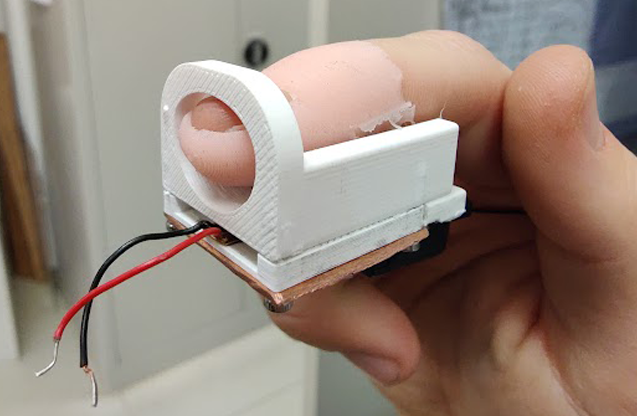
\includegraphics[width=0.2\textwidth]{Figures/rigid_prot_top.png}
        }
    \end{subcaptiongroup}
    \caption{Bottom and top view of the real prototype}
\end{figure}
This prototype is \textbf{much better} than the previous one, the \textbf{magnet} was kept \textbf{at the right distance} from the coil and the vibrations were \textbf{much more noticeable}, also being wearable made it much easier to use.
Its biggest problem was the \textbf{silicon sleeve}, as the silicon tends to \textbf{absorb some of the vibrations} and the softness of the material made the mounting mechanism a bit \textbf{unreliable}.  
We also had to add a small blowing fan to the heatsink to keep the coil cool as it would \textbf{heat a lot} after a few minutes of use.

\subsection{Flexible Mat Prototypes}
The final prototype was designed to be a \textbf{flexible silicon mat where all components were integrated}, including the membrane.

\newsavebox{\largestimage}
\begin{figure}[H]
    \centering
    \savebox{\largestimage}{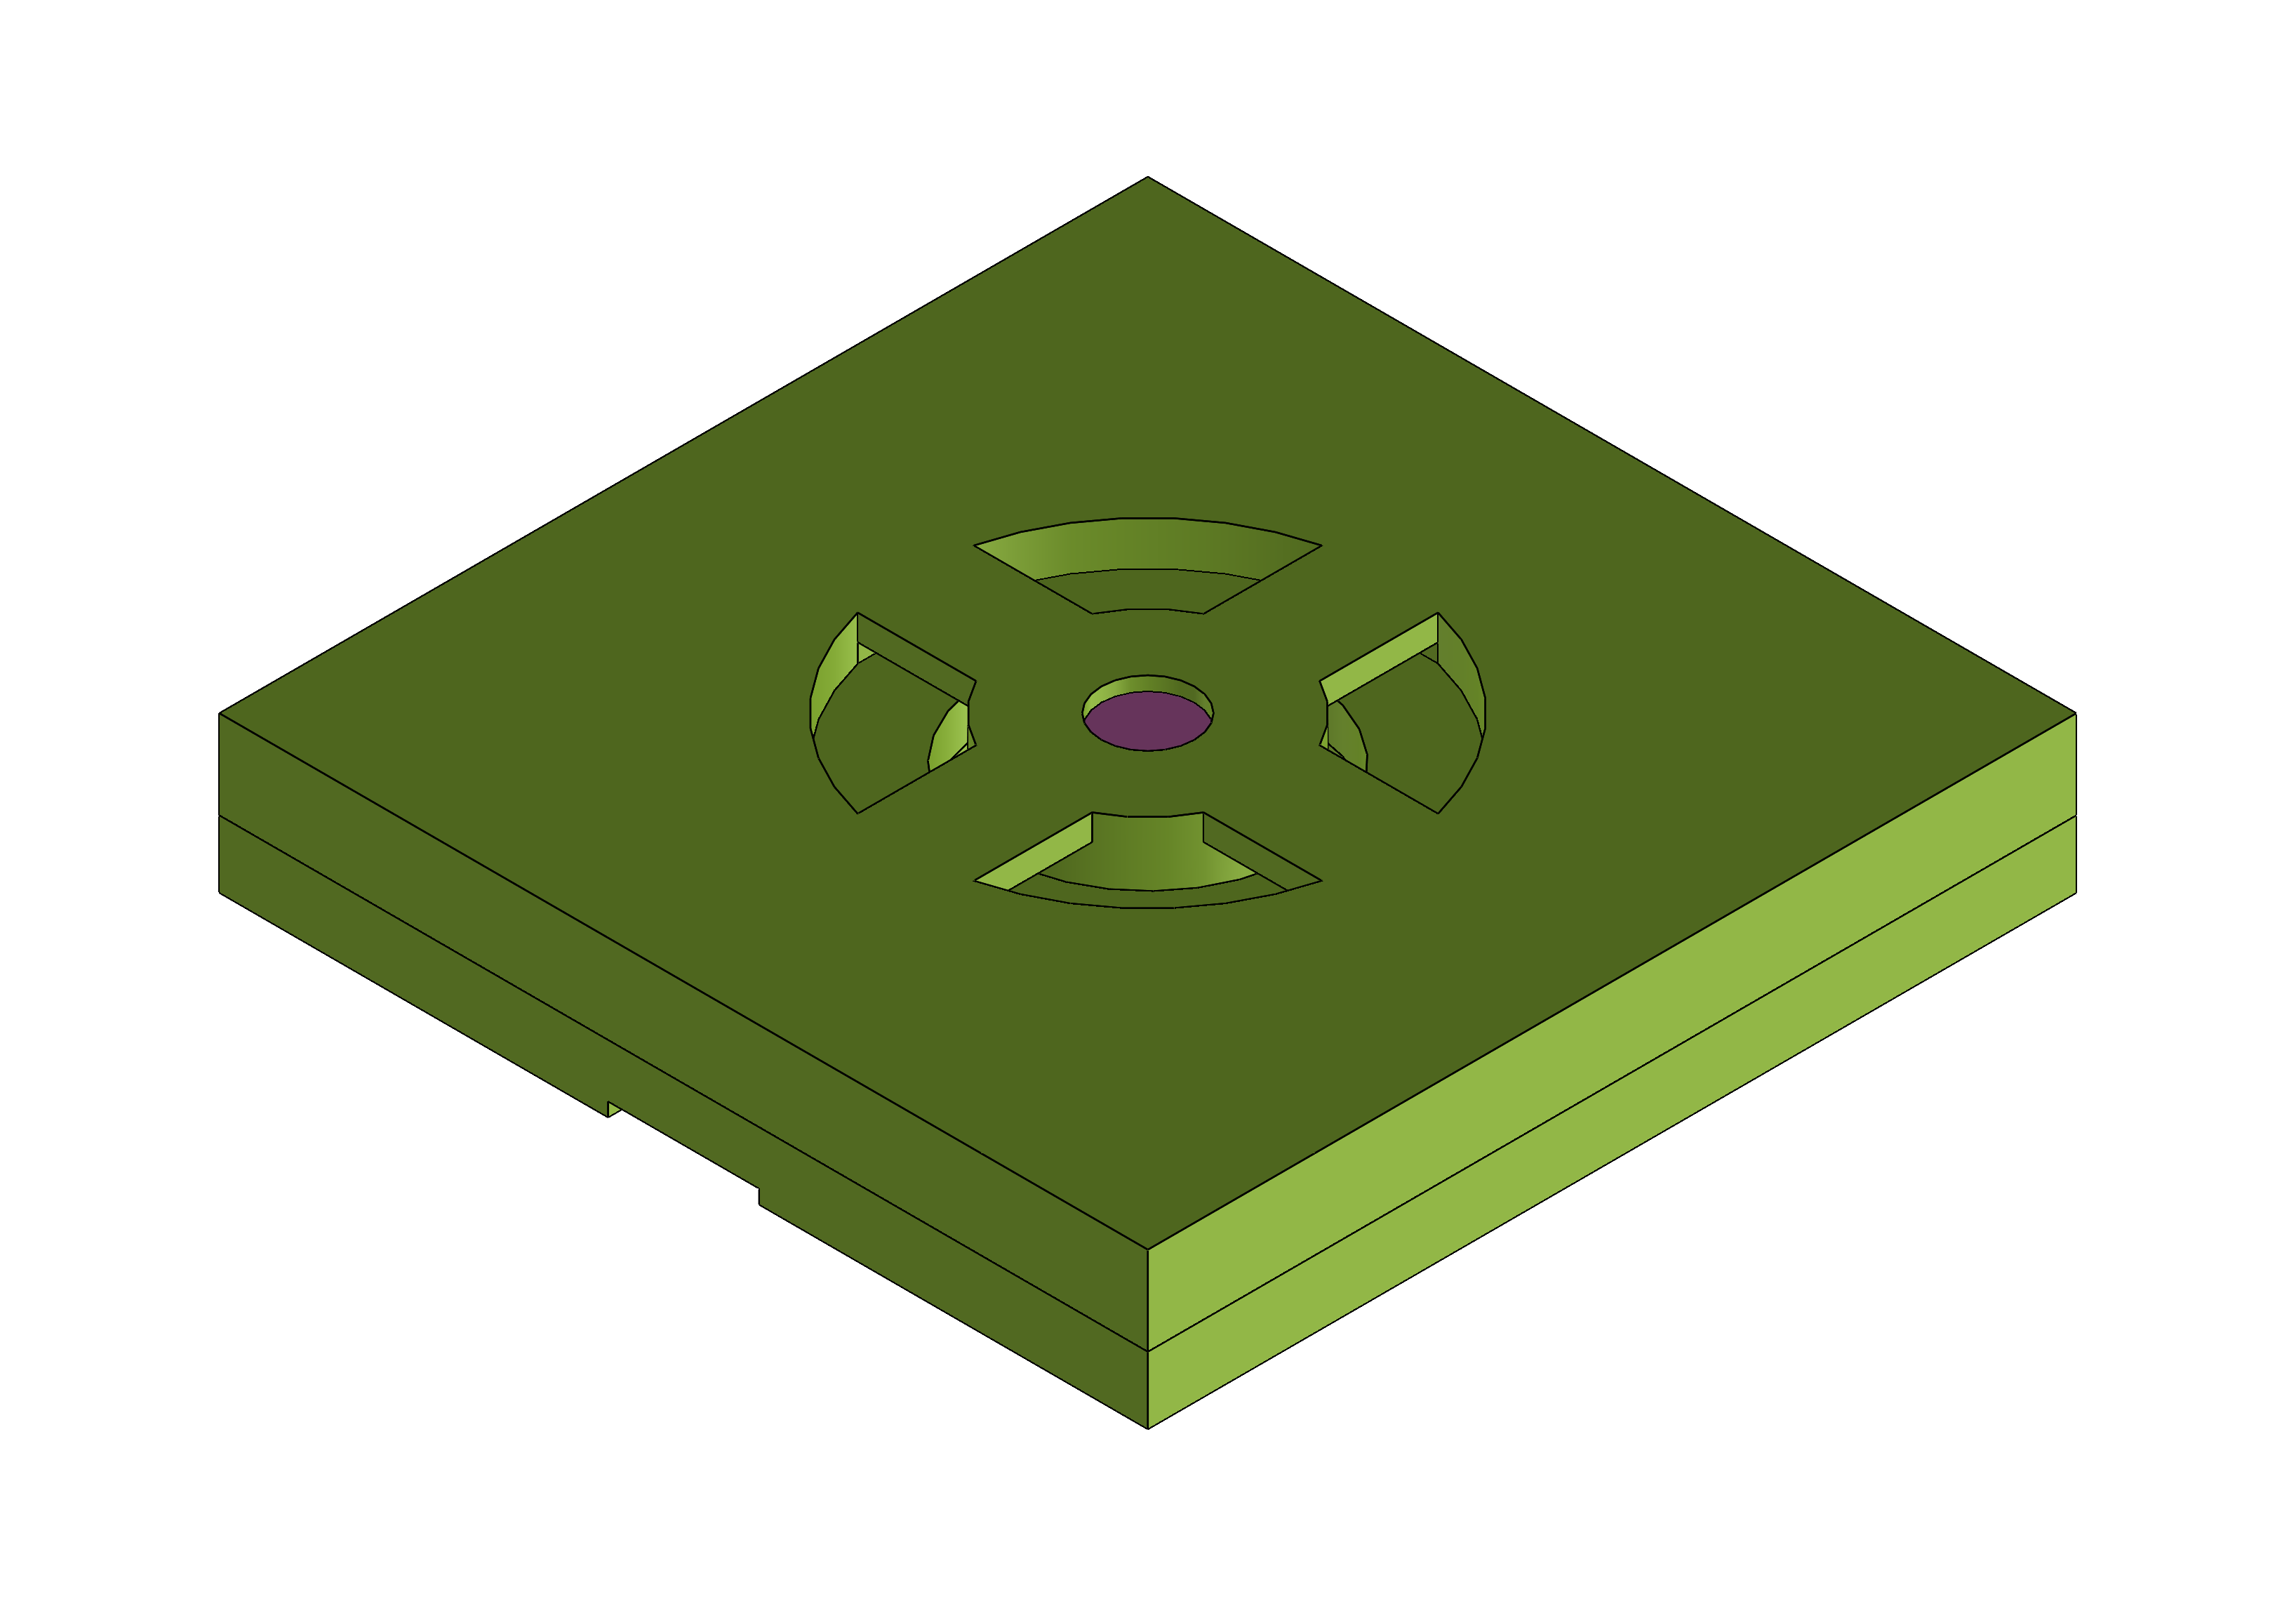
\includegraphics[width=0.2\textwidth]{Figures/membrane_v1.png}}
    \begin{subcaptiongroup}
        \centering
        \parbox[b]{0.2\textwidth}{
            \centering
            \usebox{
                \largestimage
            }
        }
        \parbox[b]{0.2\textwidth}{
            \centering
            \raisebox{\dimexpr.5\ht\largestimage-.5\height}{
                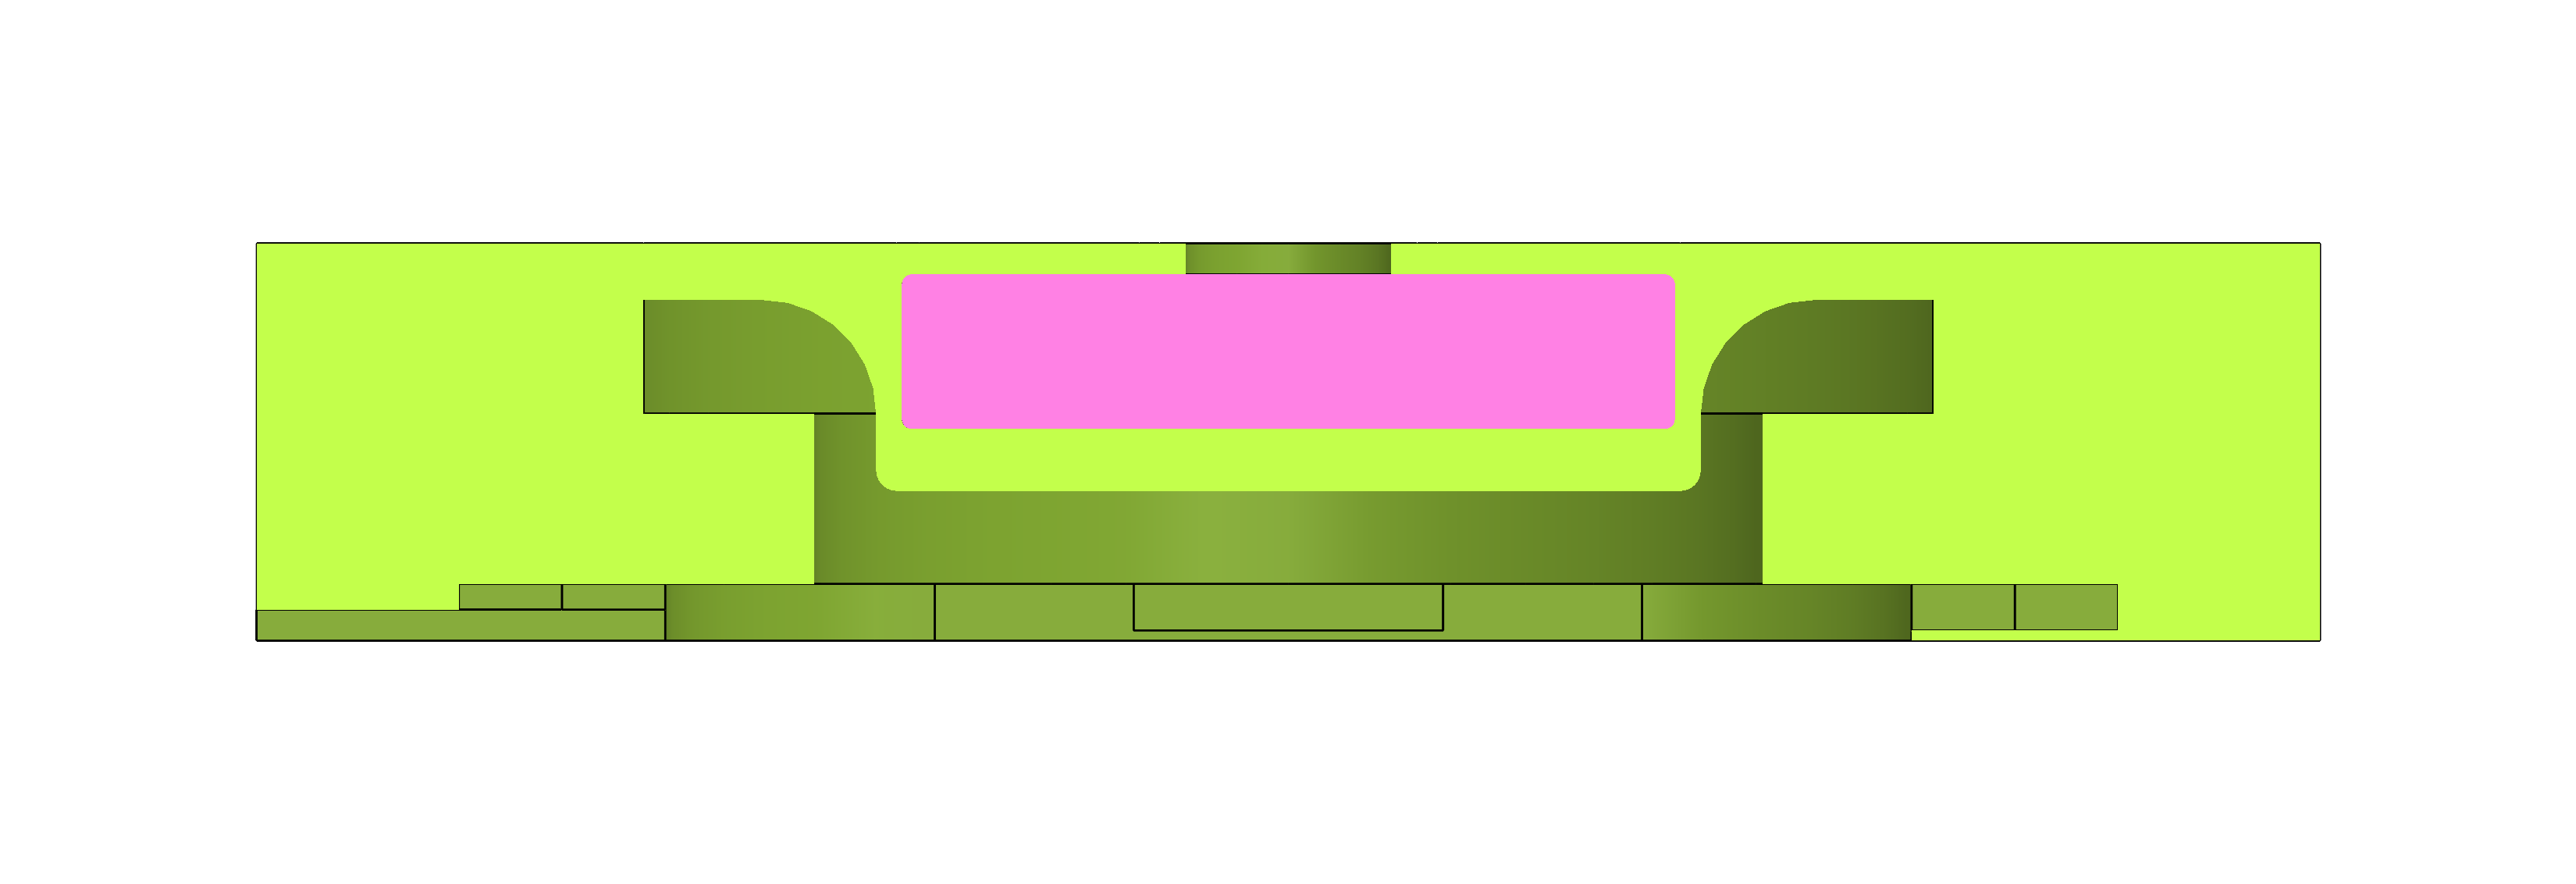
\includegraphics[width=0.2\textwidth]{Figures/membrane_v2_section.png}
            }
        }
    \end{subcaptiongroup}
    \caption{Top and section view of the flexible mat prototype}
\end{figure}
The magnet is suspended inside the silicon membrane and the coil is kept in place at the bottom of the mat.
The coil is kept inside the silicone structure thanks to a \textbf{flexible component} that is in part encased in the silicon and \textbf{acts as a trap}.

\newsavebox{\bigimage}
\begin{figure}[H]
    \centering
    \savebox{\bigimage}{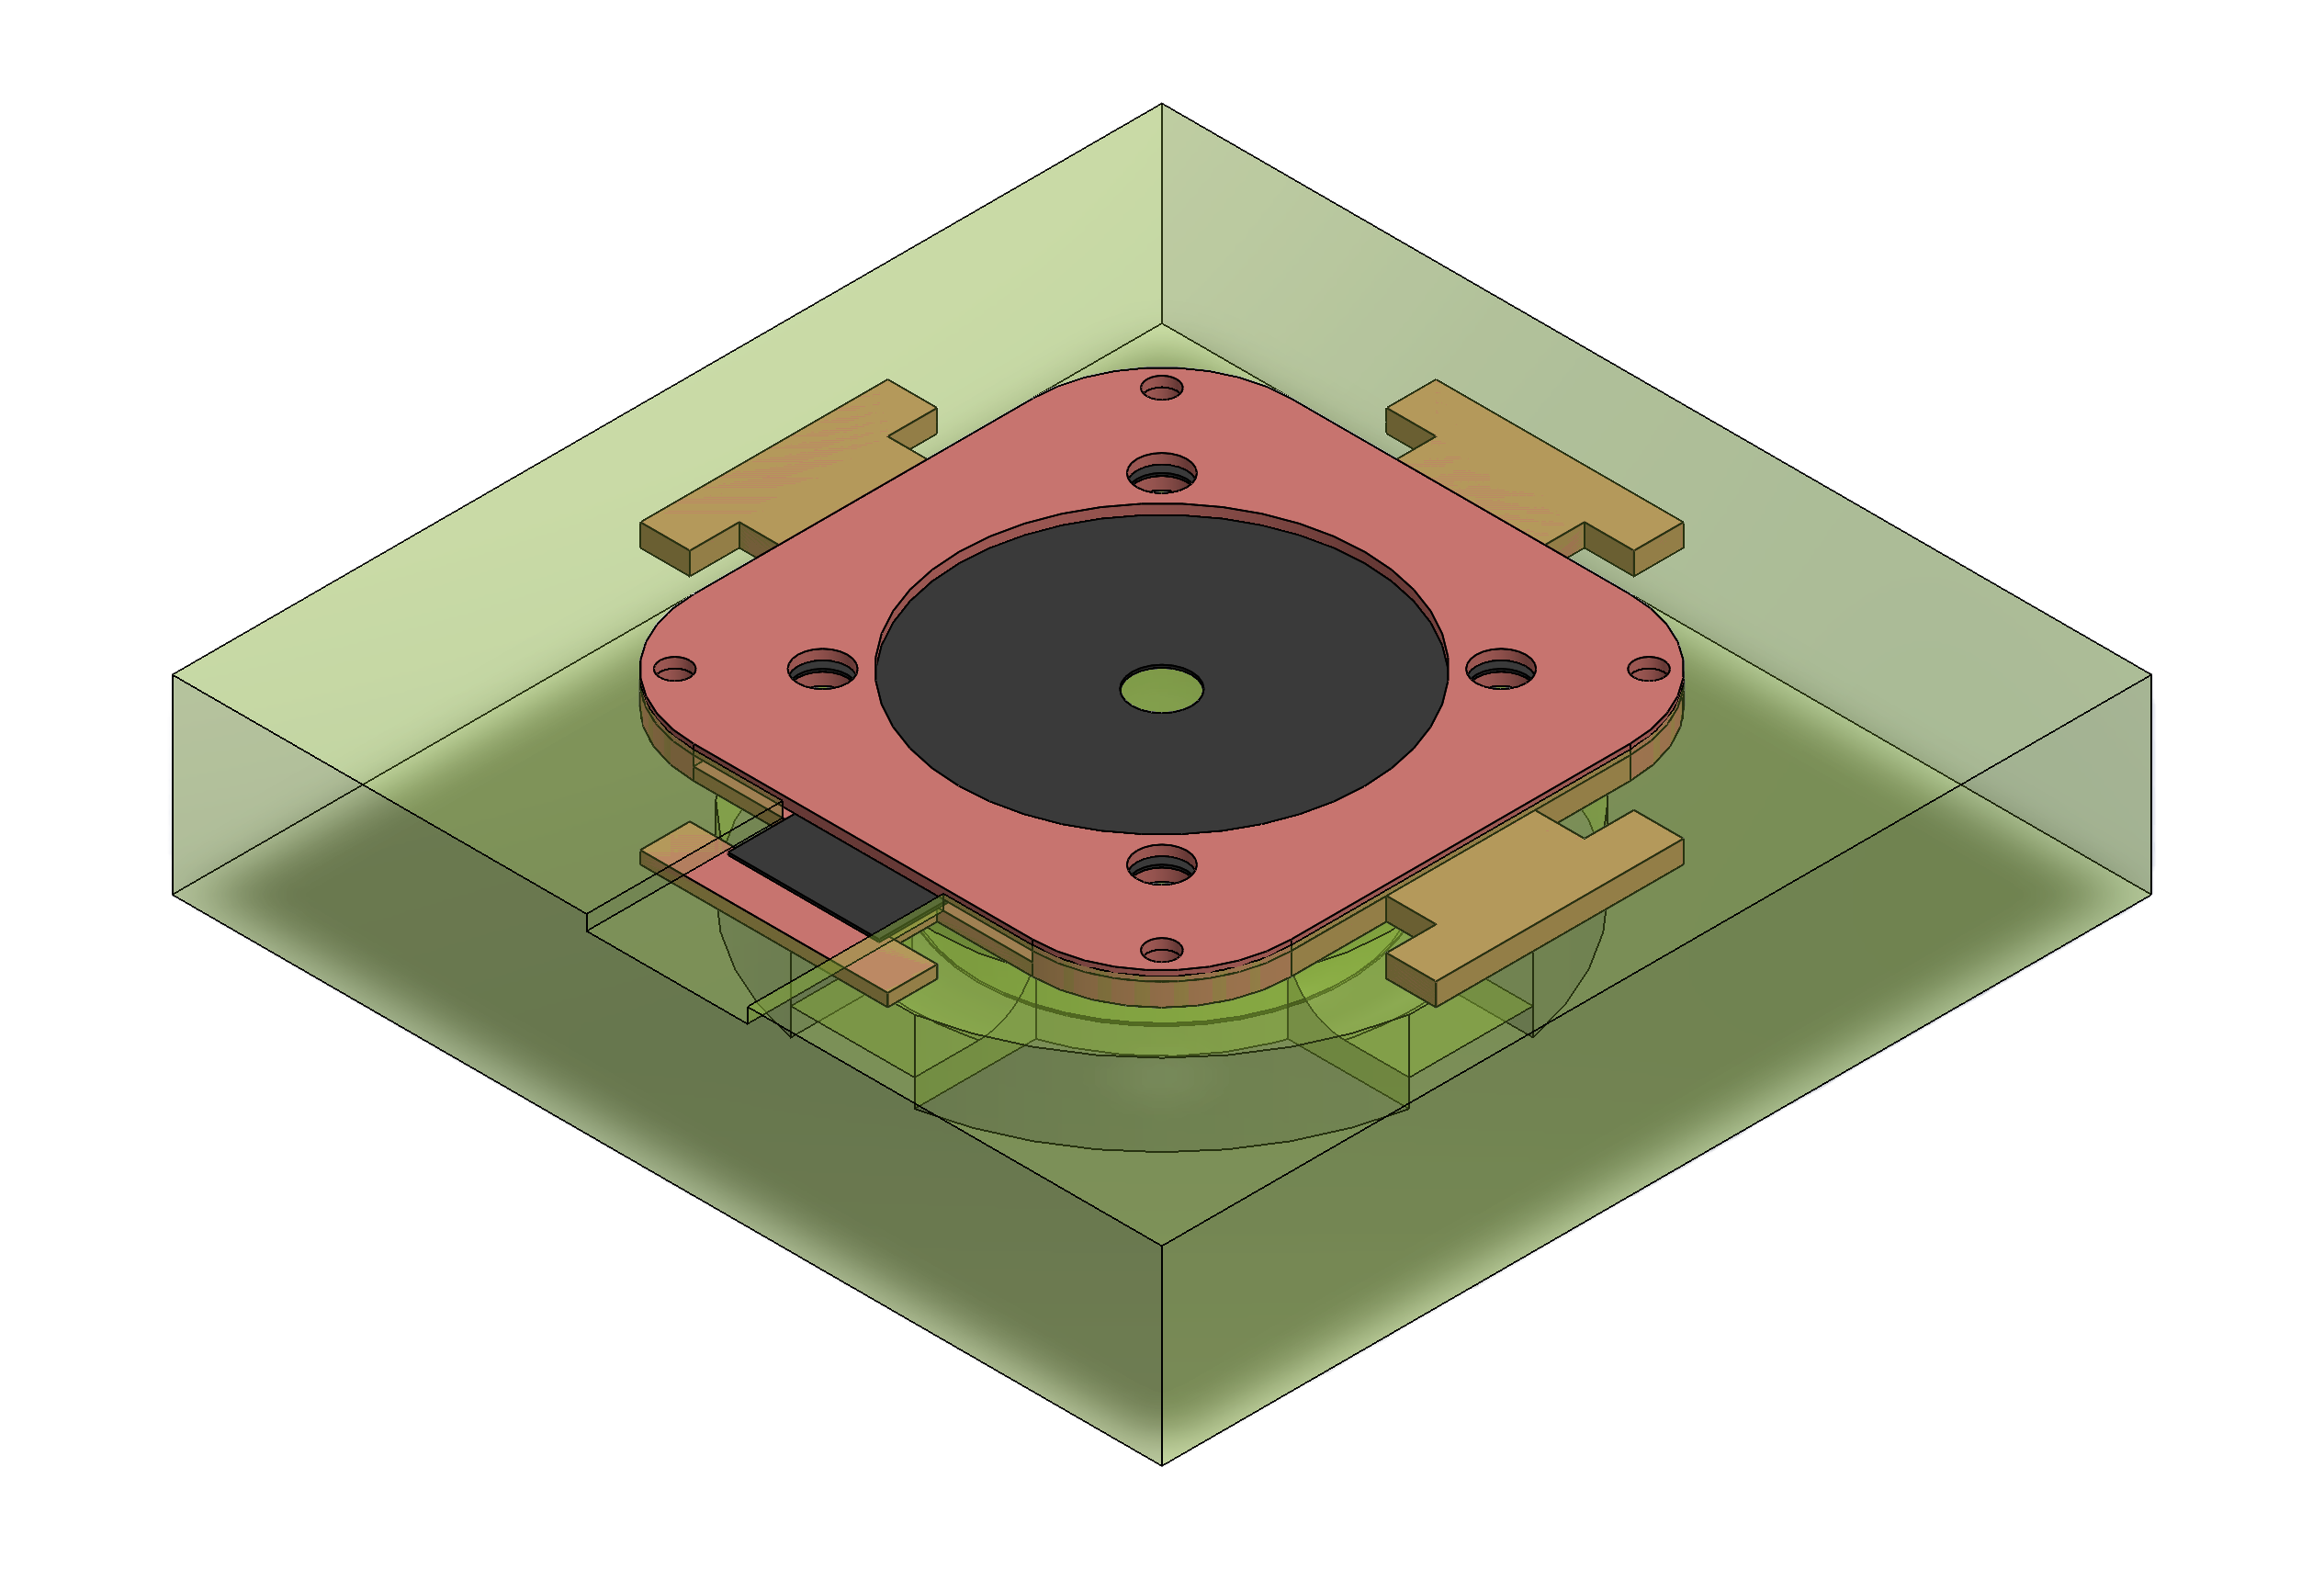
\includegraphics[width=0.2\textwidth]{Figures/coil_trap_in_mat.png}}
    \begin{subcaptiongroup}
        \centering
        \parbox[b]{0.2\textwidth}{
            \centering
            \raisebox{\dimexpr.5\ht\bigimage-.5\height}{
                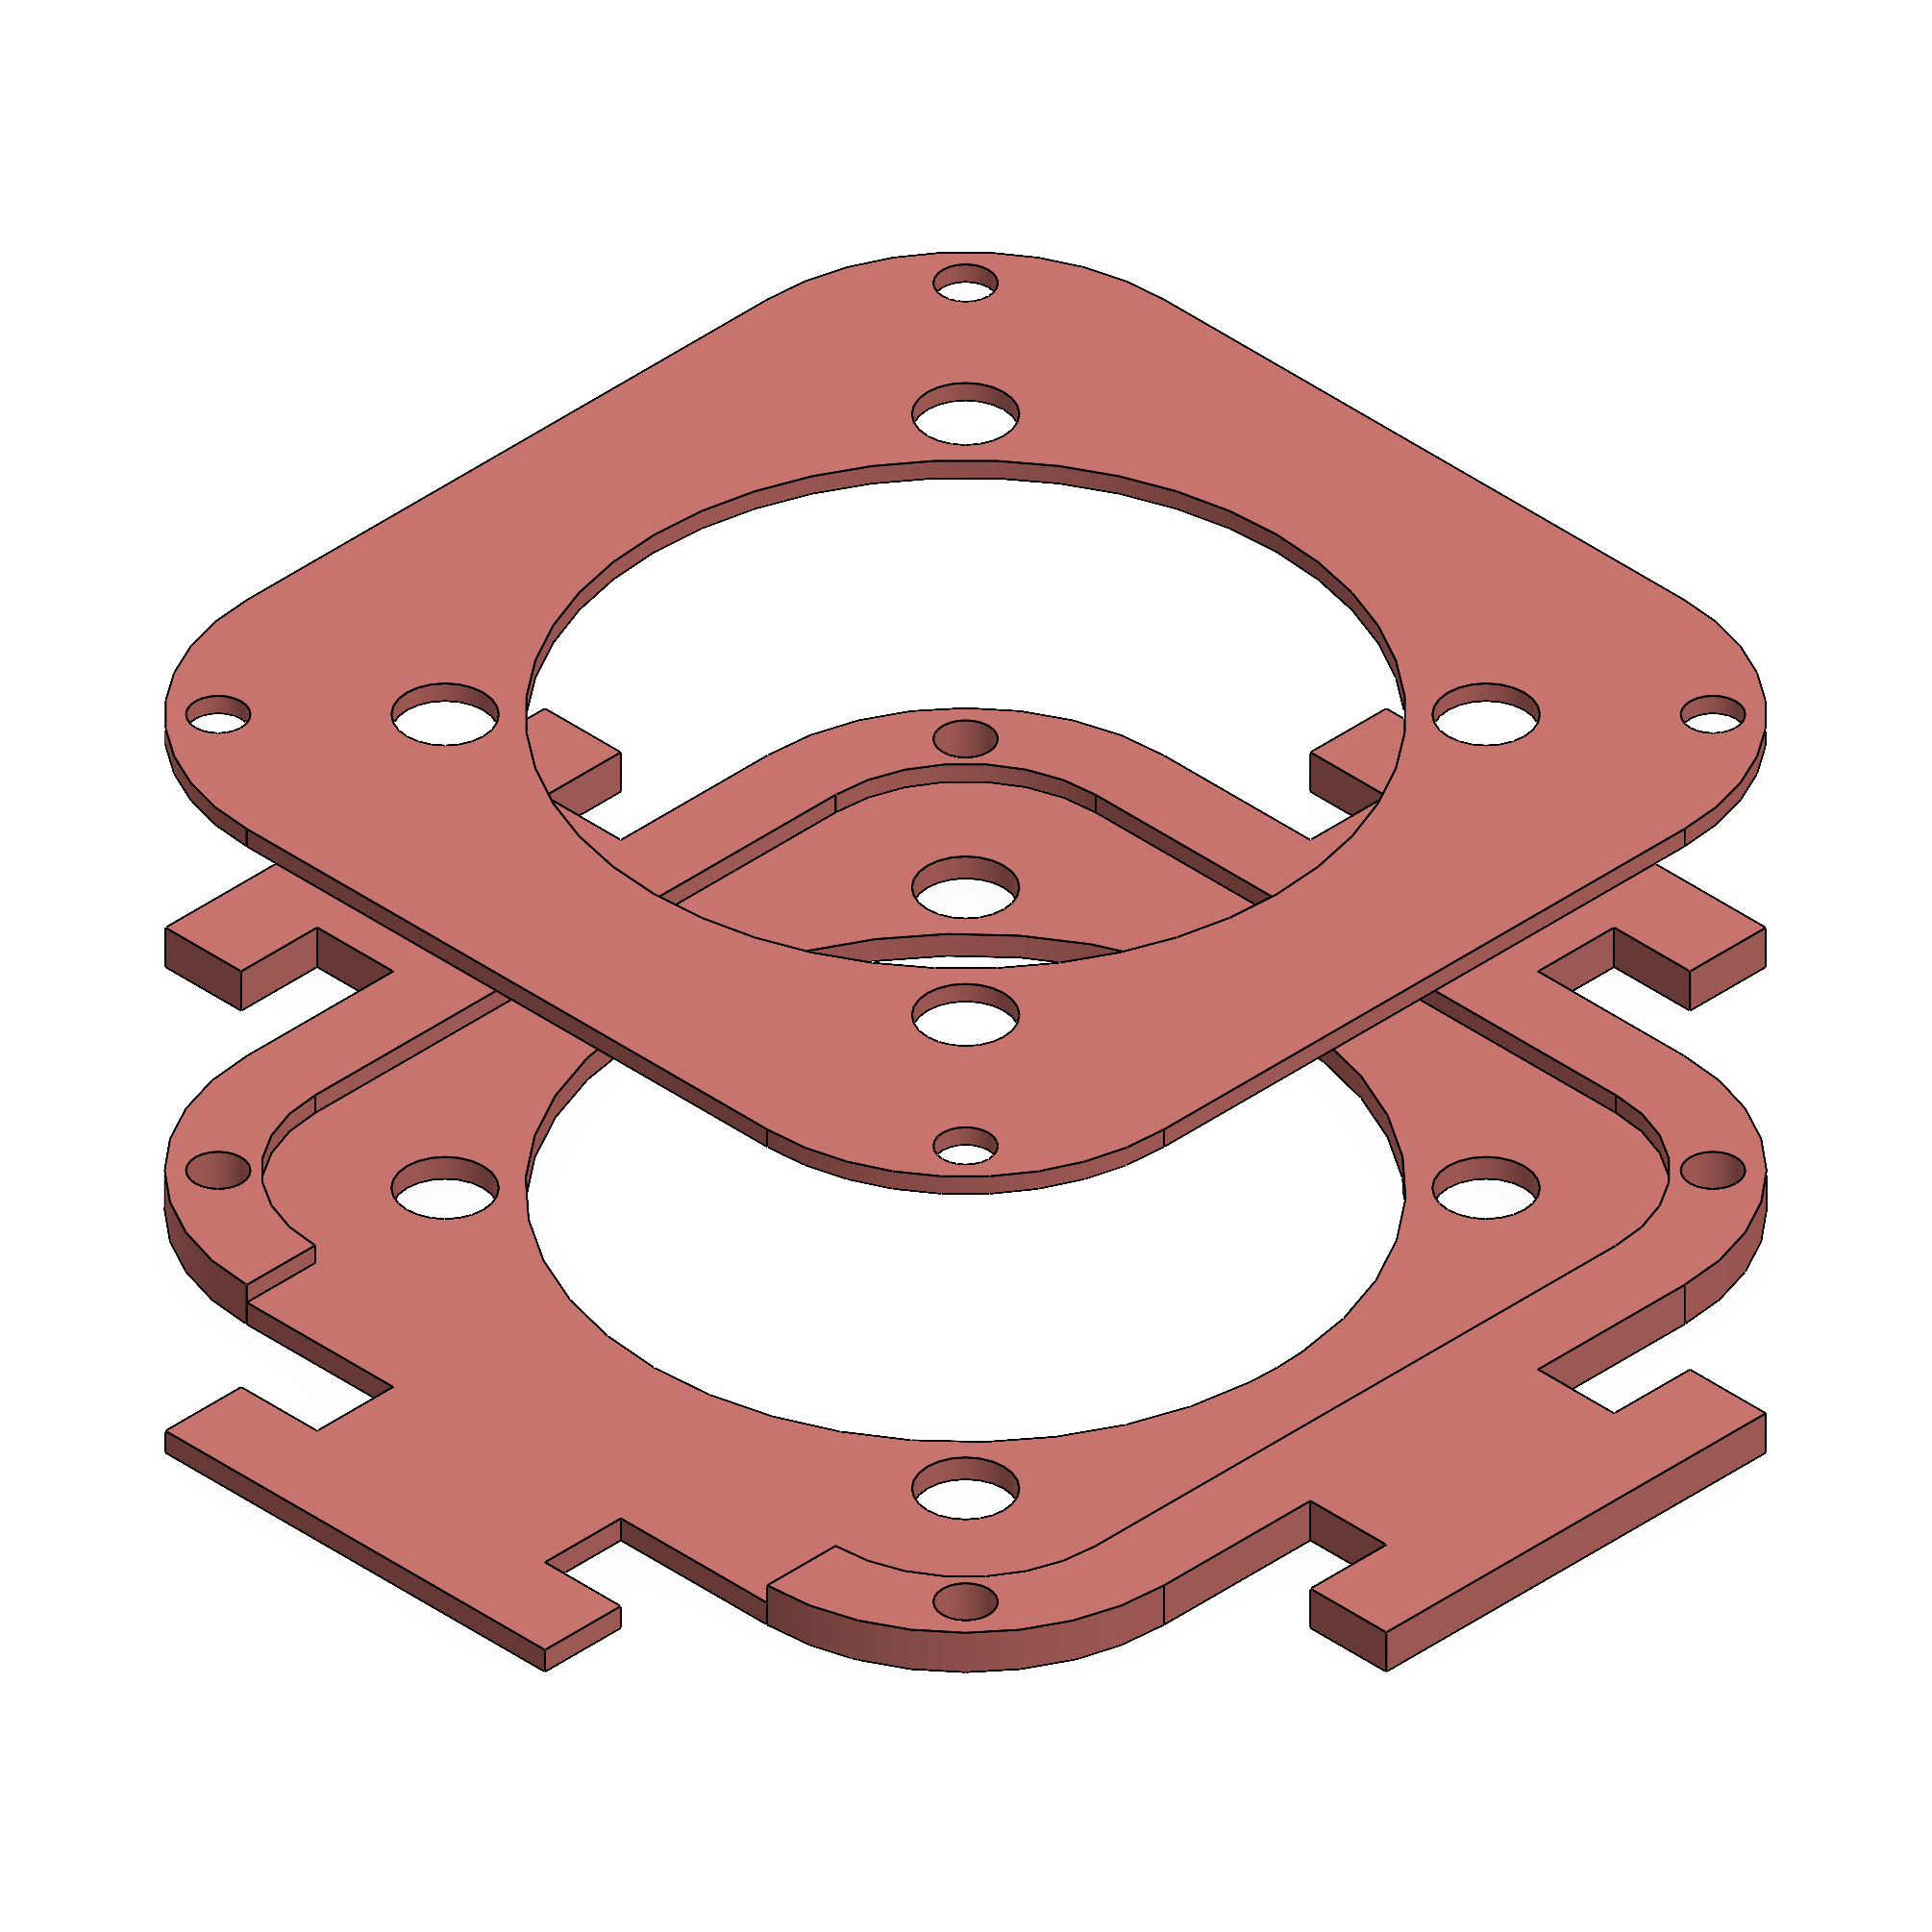
\includegraphics[width=0.15\textwidth]{Figures/coil_trap_expl.png}
            }
        }
        \parbox[b]{0.2\textwidth}{
            \centering
            \usebox{
                \bigimage
            }
        }
        
    \end{subcaptiongroup}
    \caption{Flexible coil trap.}
\end{figure}

This component allows the coil to be kept at an \textbf{optimal distance} from the magnet letting the membrane be \textbf{free to vibrate}.
This prototype resulted in the \textbf{best performances}, the vibrations were more noticeable, the mat was easy to interact with and the device could \textbf{easily flex}.
Nevertheless, we were \textbf{not still satisfied with the strength of the vibrations} it produced, the coil's problems with heating were still present and we had some \textbf{fragility problems} with the membrane and \textbf{flexing issues} with the coil trap. 

\subsection{Experimentation and Evaluation}
During our testing, we measured the \textbf{heating} production of the coil and the \textbf{force produced} by the last prototype membrane.
\subsubsection{Heating Testing}
We powered the coil with an input \textbf{voltage sweep both in DC and AC} conditions while measuring its surface temperature using a \textbf{thermocouple}. The limit of the sweep was chosen to be the maximum voltage that the coil could handle before reaching its \textbf{thermal runaway point}.
\begin{figure}[H]
    \centering
    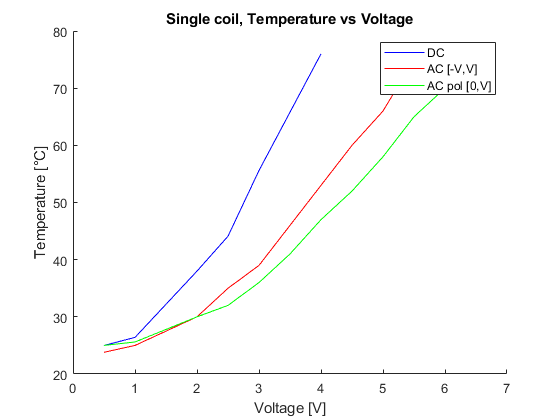
\includegraphics[width = 0.5\linewidth]{Figures/Temp_vs_Volt_1_coil.png}
    \caption{Temperature vs Voltage for one coil.}
    \label{fig: Single_coil_heating_tests}
\end{figure}
As we can observe in figure \ref{fig: Single_coil_heating_tests}, in AC conditions, especially for unipolar signals, the coil can sustain \textbf{higher voltages}; this is because sinusoidal signals have a \textbf{lower RMS} value than DC ones.

\subsubsection{Force Testing}
We measured the force produced by the membrane using an \textbf{ATI TW-Nano17 force sensor}. The prototype's coil was powered with a \textbf{heartbeat-like signal}, as it's a \textbf{very low RMS} signal that allows us to run the coil at \textbf{30V peak voltage}.
This was necessary because the sensor \textbf{sensitivity was too low} to measure the force produced by sinusoidal signals at \textbf{6V}.
\begin{figure}[H]
    \centering
    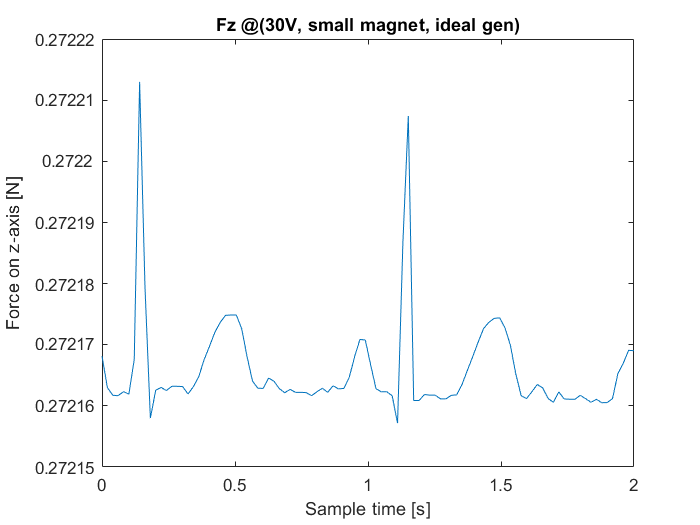
\includegraphics[width = 0.5\linewidth]{Figures/Fz_@30V_small_magn_idealgen.png}
    \caption{Force profile of the generated by the heartbeat signal.}
    \label{fig: Force_profile}
\end{figure}
From figure \ref{fig: Force_profile} we can observe that the membrane produces a \textbf{constant force of about 0.2N}, due to the silicone membrane itself, and the \textbf{net force} produced by the coil at the peak of the signal is in the order of \textbf{$5\cdot10^{-5}$N}.

\section{Conclusions}
\subsection{Low force Output}
In the previous chapter, we measured the \textbf{maximum force} our system could generate in the \textbf{best conditions}.
Even by \textbf{overloading} the coil with short bursts of 30V it couldn't generate \textbf{enough force} to reach the \textbf{haptic sensitivity of human fingers}. Test subjects were anyway able to feel some vibrations, we can theorize that the sensitivity \textbf{threshold was lowered by the constant pressure} force applied on the skin by the membrane.
Even still the vibrations were \textbf{very weak} and \textbf{barely perceptible}.
\subsection{A technology not suitable for haptic feedback devices}
Driving flexible coils with \textbf{AC signals} is very \textbf{difficult} and \textbf{inefficient}.
The complex circuitry required to drive these coils is not only \textbf{expensive} but also \textbf{difficult to design and tune}.
The high power consumption is also a major drawback.
Combining all these factors with the low magnetic field output, we can conclude that this technology is \textbf{not ready for mainstream application in haptic feedback devices}.

\end{document}